\chapter{Espaços Vetoriais}
Começaremos pela definição de um espaço vetorial, onde, podemos tratar como um vetor ao designar um elemento do espaço vetorial de um número $\mathbb{R}$ definido tal que:

\noindent\textbf{Definição 01:} Seja um conjunto V, não vazio, com duas operações: soma, $V \times V \rightarrow V$, e multiplicação por escalar, $R \times V \rightarrow V$, tais que, para quaisquer $u, v, w \in \mathbb{R}$, satisfaçam as propriedades: \nocite{boldrini1980}
\begin{enumerate}
	\item $(u + v) + w = u + (v + w), \forall$ $u, v, w \in V$ (propriedade associativa.) 
	\item $1u = u$.
	\item $u + v = v + u, \forall$ $u, v \in V$ (propriedade comutativa).
	\item $\exists$ $0$ $\in V$ tal que $u + 0 = u$.
	\item $\exists$ $-u \in V$ tal que $u + (-u) = 0$.
	\item $a(u + v) = au + av$.
	\item $(a + b)v = av + bv$.
	\item $(ab)v = a(bv)$.
	\item $1u = u$.
\end{enumerate}

\noindent\textbf{Observação:} $\textbf{0}$ é o vetor nulo. \nocite{ulhoa2018}

\noindent\textbf{Observação:} Limitaremos nossa discussão, demonstrações e aplicações dentro do conjunto dos números reais apenas.

\noindent\textbf{Exemplo 01:} Suponhamos uma matriz $M_{(2, 2)}$, onde, é denotado por $M_{(m,n)}$, dado por $M = [a_{ij}]_{m \times n}$ podendo ser interpretada dessa forma, $V = M_{(2, 2)}$, onde $V$, é um conjunto não vazio, seu escalar pertencente ao conjunto dos $\mathbb{R}$, que satisfazem todas as propriedades de um espaço vetorial.

\begin{figure}[H]
	\centering
	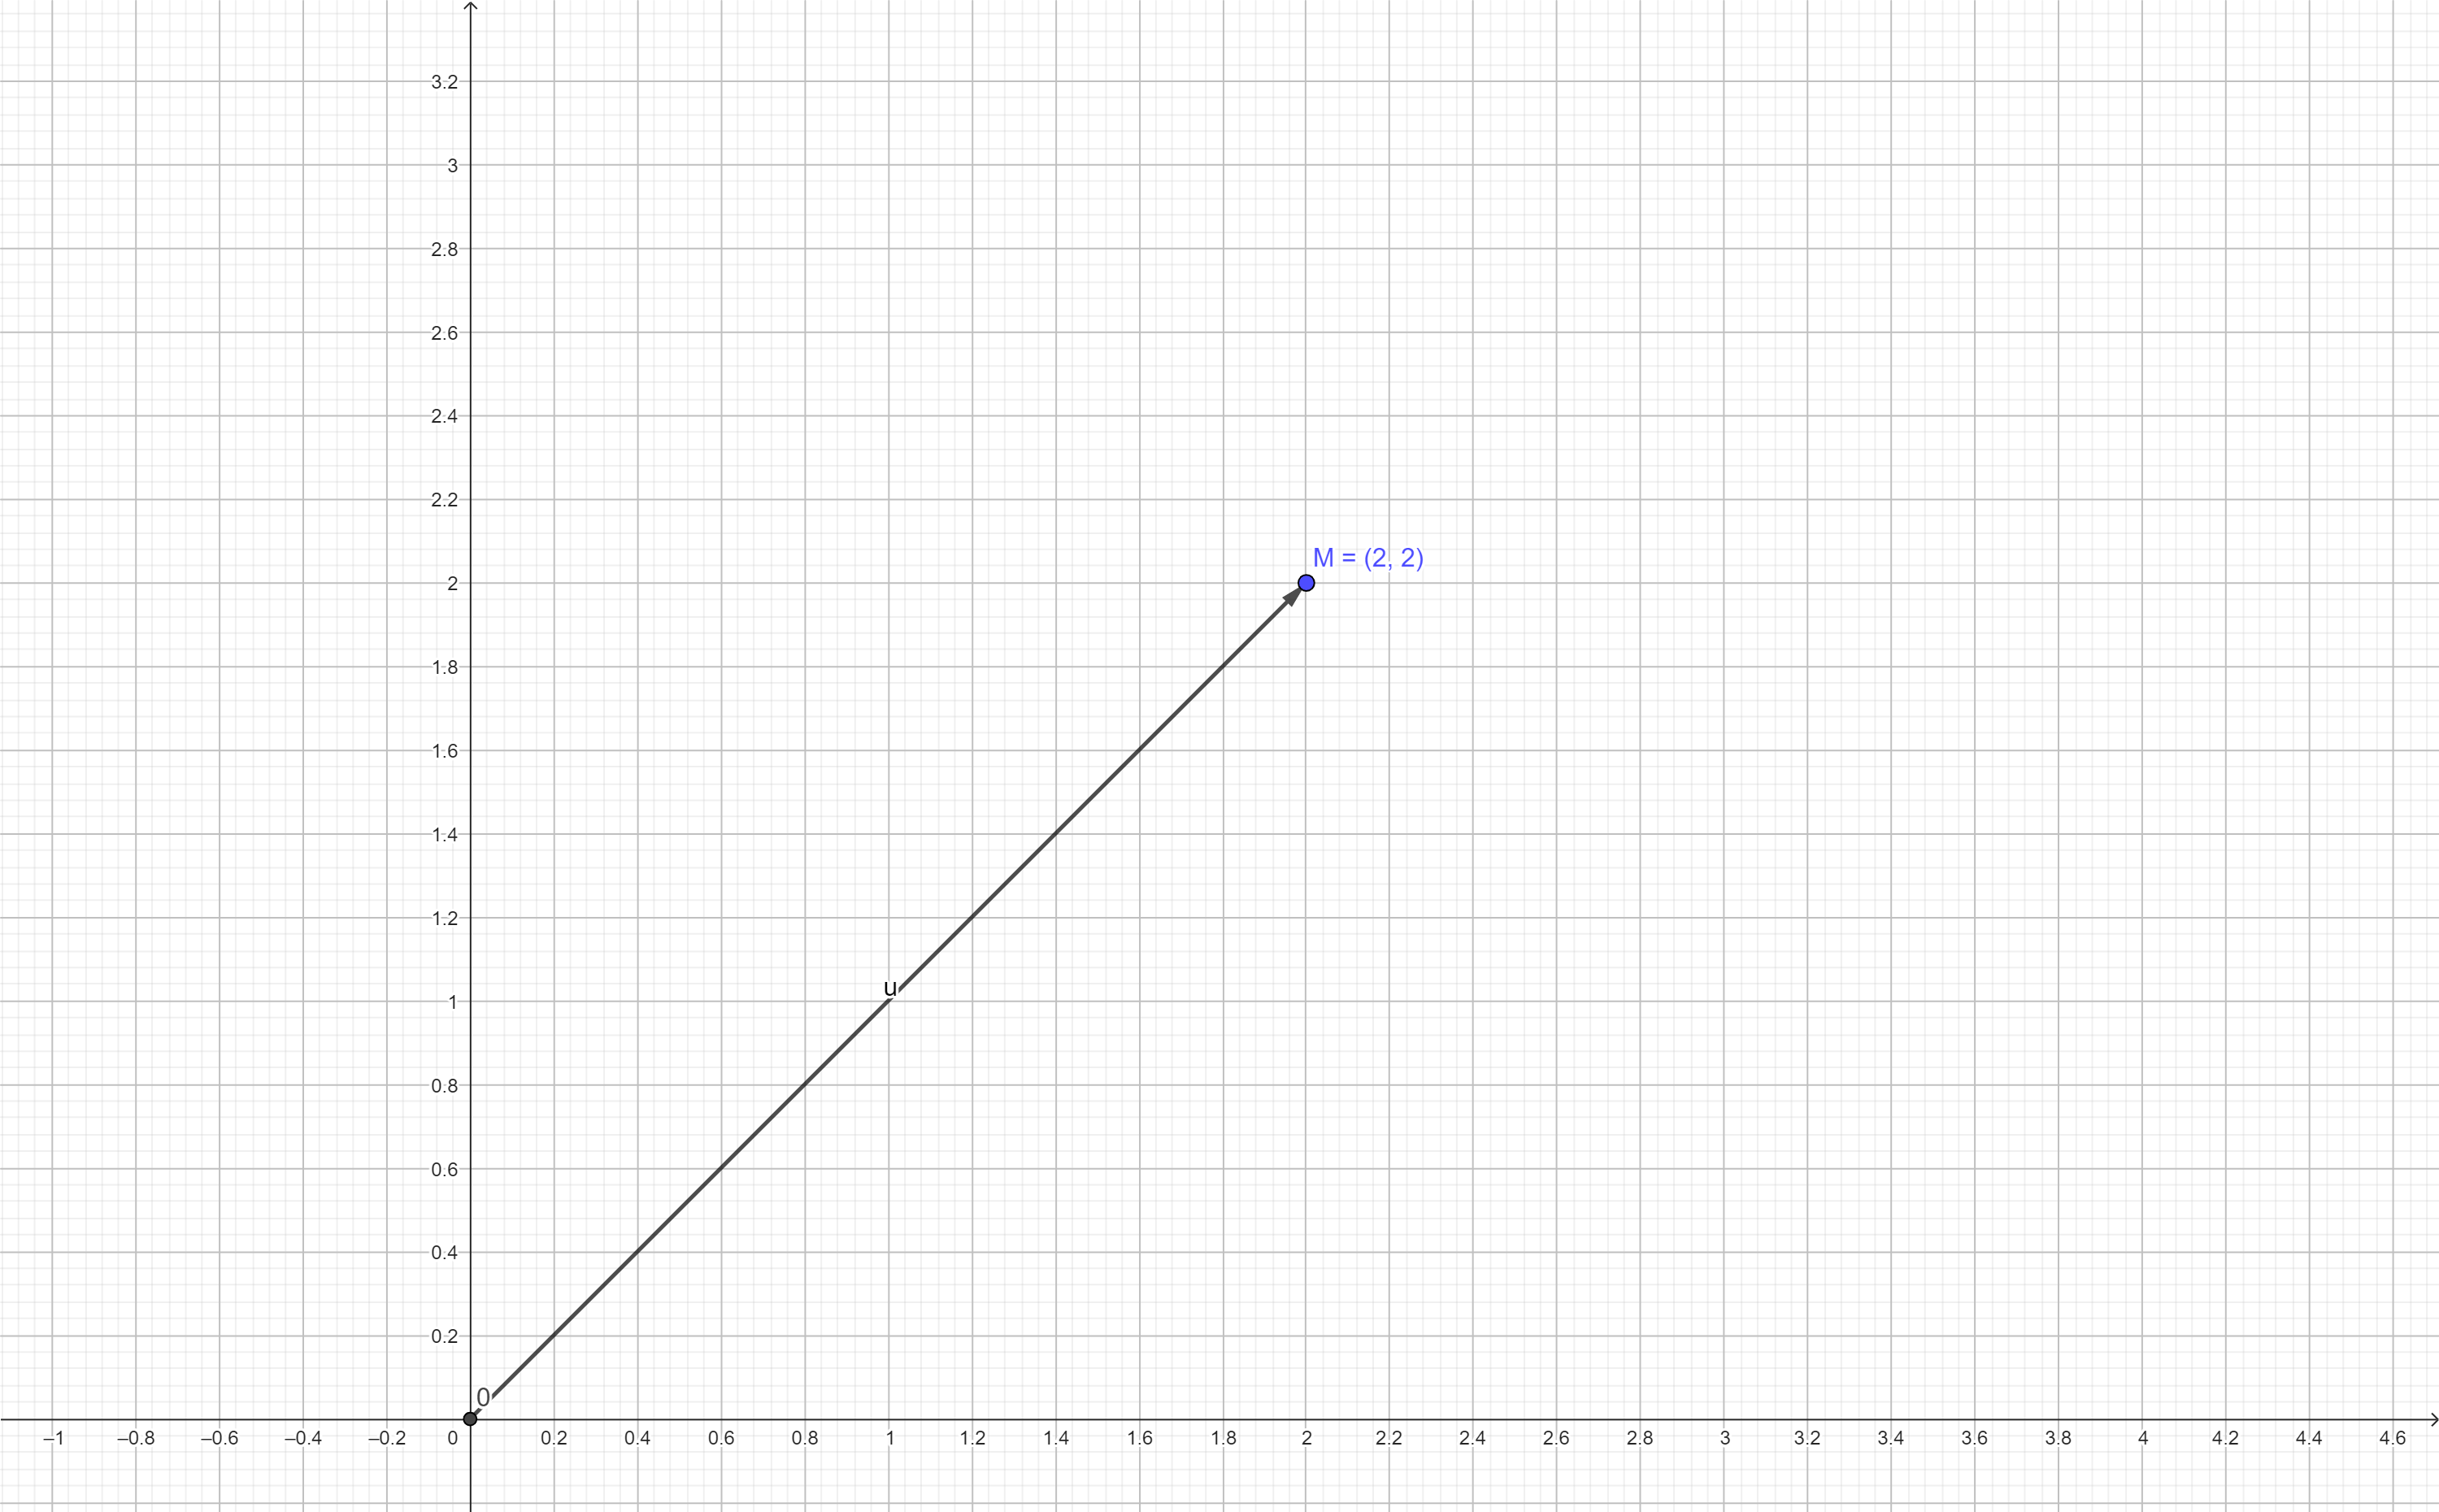
\includegraphics[scale=1.0]{exemplo01.png}
	\caption{Exemplo 01: Vetor no plano.}
\end{figure}

A partir disso, podemos perceber o uso analítico dos espaços vetoriais para resolução de problemas em geral. Vejamos mais alguns exemplos.

\noindent\textbf{Exemplo 02:} O exemplo anterior, trata-se de uma matriz de $\mathbb{R}^2$ pode ser dito como, no plano, agora iremos expandir para $\mathbb{R}^3$, seja um vetor $A = (x, y, z)$ ou representado pela forma matricial:

\[
A = \begin{bmatrix}
	a \\ b \\ c
\end{bmatrix}
\]
\noindent Assim, por quaisquer números reais, podemos fazer uma projeção ortogonal no espaço, segue um exemplo traçado:

\begin{figure}[H]
	\centering
	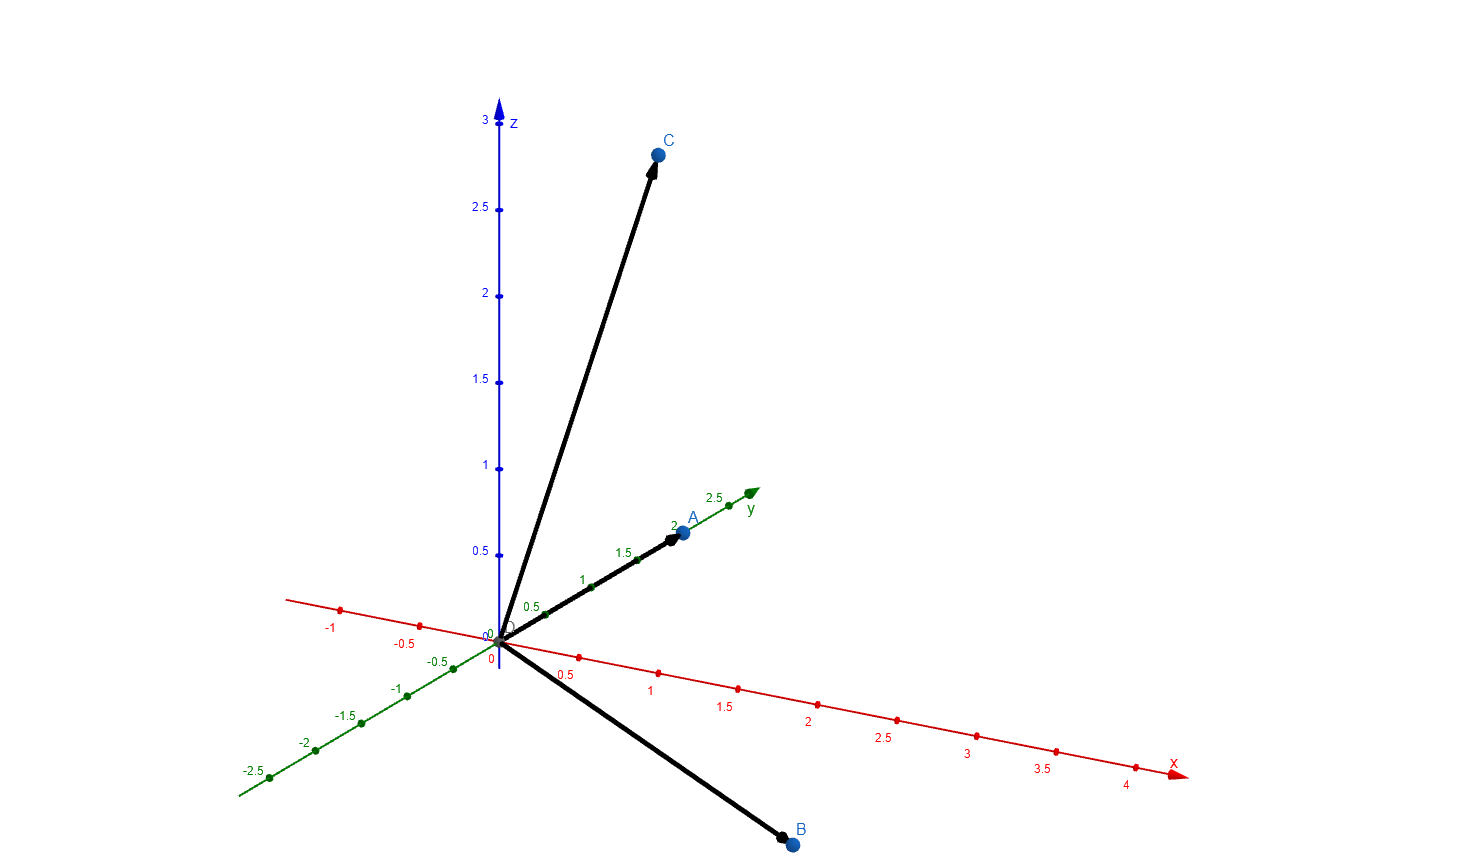
\includegraphics[scale=0.30]{exemplo02.png}
	\caption{Exemplo 02: Exemplo de vetor no espaço.}
\end{figure}

\noindent\textbf{Exemplo 03:} Consideremos $n-uplas$ de números reais.

$V = \mathbb{R}^n = {(x_1, x_2, \ldots, x_n); x_i \in \mathbb{R}}$

e se $u = (x_1, x_2, \ldots, x_n), v = (y_1, y_2, \ldots, y_n)$ e $a \in \mathbb{R}$,

$u + v = (x_1 + y_1, x_2, y_2, \ldots, x_n, y_n)$ e $au = (ax_1, ax_2, \ldots, ax_n)$

Por tratarmos de uma quantidade $n$ de números, o campo tridimensional deixa de ser visto, e passamos a ter $\mathbb{R}^n$ dimensões, as propriedades não deixam de valer independente a quantidade de dimensões.

% SubEspaço vetorial
\section{Subespaços Vetoriais}
Nesta seção iremos introduzir conceitos no estudo de espaço vetorial para subespaço vetorial.

\noindent\textbf{Definição 02:} Dado um espaço vetorial V, um subconjunto W, não vazio, será um subespaço vetorial de V se:
\begin{enumerate}
	\item Para quaisquer $u, v \in W$ tivermos $u + v \in W$.
	\item Para quaisquer $a \in R, u \in W$ tivermos $au \in W$.
	\end{enumerate}

\noindent\textbf{Teorema 01:} Um subconjunto não vazio $W$ de $V$ é um subespaço de $V$ se, e somente se, para cada par de vetores $\alpha, \beta$ em $W$ e cada escalar $c$ em $F$, o vetor $c\alpha + \beta$ está em $W$.

\noindent\textbf{Demonstração:} Suponhamos que $W$ seja um subconjunto não vazio de $V$ tal que $c\alpha + \beta$ pertença a $W$ para todos os vetores $\alpha$, $\beta$ em $W$ e todos escalares $c$ em $F$. Como $W$ é não vazio, existe um vetor $\rho$ em $W$, logo $(-1) \rho + \rho = O$ está em $W$. Então se $\alpha$ é um vetor arbitrário em $W$ e $c$ é um escalar arbitrário, o vetor $c\alpha = c\alpha + O$ está em $W$. Em particular $(-l)\alpha = -\alpha$ está em $W$. Finalmente se $\alpha$ e $\beta$ estão em $W$, então $\alpha + \beta = l\alpha + \beta$ está em $W$.
Assim, $W$ é um subespaço de $V$. \nocite{hoffman1979}

\noindent\textbf{Exemplo 04:} Considere o espaço vetorial $\mathbb{R}^3$. O conjunto de todos os vetores que residem no plano $xy$, ou seja, ${(x, y, 0) \mid x, y \in \mathbb{R}}$, forma um subespaço vetorial de $\mathbb{R}^3$. Verifique as propriedades de um subespaço vetorial para confirmar isso.

\noindent\textbf{Exemplo 05:} No espaço vetorial das funções reais de uma variável real, $V = {f(x) \mid f: \mathbb{R} \rightarrow \mathbb{R}}$, considere o conjunto de todas as funções lineares, ou seja, ${f(x) = mx + b \mid m, b \in \mathbb{R}}$. Esse conjunto forma um subespaço vetorial de $V$. Novamente, você pode verificar as propriedades para confirmar.

\noindent\textbf{Exemplo 06:} No espaço das matrizes reais $2 \times 2$, $M_{(2,2)}$, considere o conjunto de todas as matrizes simétricas, ou seja, aquelas em que $A = A^T$. Esse conjunto forma um subespaço vetorial de $M_{(2,2)}$. Você pode demonstrar isso verificando as propriedades de um subespaço vetorial

% _{m \times n}

% subinscrito
% _
% expoente com mais de um dígito
% x^{21}
